Our system consists of two major components: an automatic mesh generator and an interactive model editor.

The mesh generator can procedurally generate a realistic clay mesh by adding Perlin Noise. With the interactive pottery model editor, the user can shape the virtual clay in real time intuitively to design virtual pots.

The virtual pots created by our system can be exported as OBJ files and used for 3D printing.

The results of our user study has shown that our system requires lower cognitive load compared with desktop modeling experience and allows more creativity than touchscreen-based interfaces. Users without real-life pottery experience and 3D modeling knowledge can easily create virtual pottery works with our system.

//background - CAD
In recent years, emerging technologies such as 3D printing introduces a new way of pot design, enabling people to fabricate pots in a digital way with the help of Computer Aided Design (CAD) software and 3D printers.

// pottery 
As one of the oldest inventions in human history, pottery has drawn much interests, leading to the emergence of virtual pottery systems.




// This model is the "basic haptic model" and an advanced model is presented in the next section.

///////////////////////////////////////////////////////


\subsection{User Study 3: RealPot vs other cad system}
\label{sec:study3}
%GOAL
%RealPot vs Maya
To investigate the influence of modeling pipeline, we compare RealPot and Autodesk Maya since they both support 3D modeling. They differ in workflow to create and edit meshes. While RealPot can automatically generate a mesh for deformation with motion controllers, Maya needs to create a mesh from a primitive cylinder in order to edit in vertex mode, edge mode or face mode with mouse and keyboard. 
%RealPot vs Lets
On the other hand, RealPot and LCP have similarities in their workflows with intuitive interactions. They both allow users deform the mesh interactively with natural user interfaces. While RealPot enables parameter control and spatial interaction, LCP has no parameter control and provides touchscreen-based experience.

\subsubsection{Evaluated Systems}

The three evaluated systems were as follows:

\paragraph{RealPot}: Our virtual pottery tool based on HTC Vive VR system. The user can shape the virtual clay with bimanual spatial interactions.
\paragraph{Let’s Create! Pottery}: A touchscreen-based pottery creation tool on mobile devices. Users can interactively create pottery models by finger swiping on the screen.
\paragraph{Autodesk Maya}: A traditional desktop 3D modeling system, which provides a set of powerful tools for professional 3D artists. The user can edit vertex, edge, face etc. with mouse and keyboard.

The interfaces of all the three systems are demonstrated in Figure \ref{fig:sys}, and a comparison of interactions in these systems is listed in Table \ref{tab:3}. 
Although the three systems are different, we focus on comparing them based on their similarities and workflows.

%%%Fig%%% Sys
\begin{figure*}
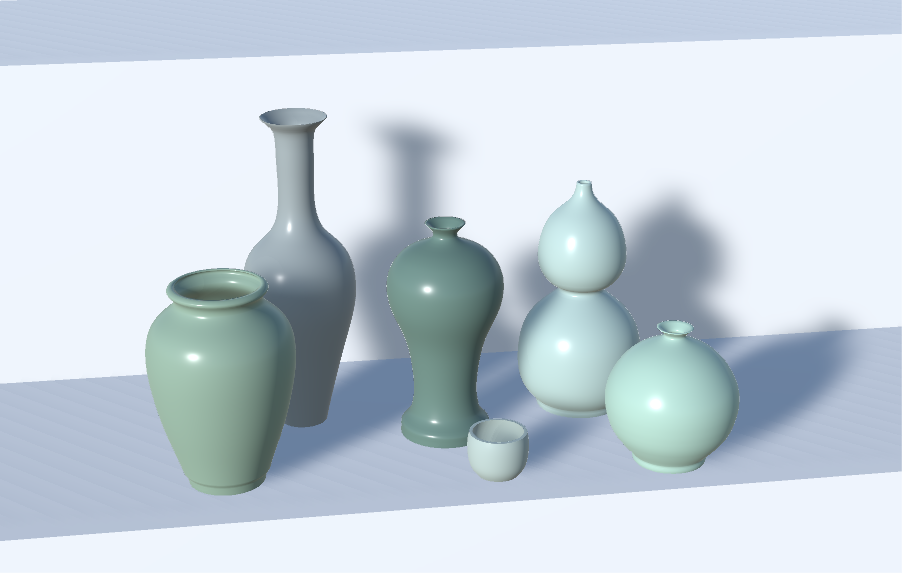
\includegraphics[width=\textwidth]{fig11}
\caption{The three systems used in our user study. (a) A virtual reality system RealPot proposed by us. (b) A touchscreen-based system Let's Create! Pottery. (c) A desktop modeling tool Autodesk Maya.}
\label{fig:sys}
\end{figure*}

% For tables use
\begin{table}
% table caption is above the table
\caption{A comparison of interactions in the three systems used in our user study.}
\label{tab:33}       % Give a unique label
% For LaTeX tables use
\begin{tabular}{llllll}
\hline\noalign{\smallskip}
System & Platform & Input Method & Head Tracking & Stereoscopy & 2D or 3D UI \\
\noalign{\smallskip}\hline\noalign{\smallskip}
RealPot & PC & Hand-held Motion Controllers & Yes & Yes & 3D \\
LCP & iPad & Touchscreen & No & No & 2D \\
Maya & PC & Keyboard and Mouse & No & No & 2D \\
\noalign{\smallskip}\hline
\end{tabular}
\end{table}

\subsubsection{Participants}
19 participants were participated in our user study, 10 males and 9 females, whose age ranged from 8 to 32 years. 8 of the subjects are familiar with VR systems (42.1\%); 2 of the subjects have experience with 3D modeling tools (10.5\%); 4 of the subjects have amateur pottery throwing experience in real life (21.1\%).
%Figure \ref{fig:11} shows two subjects using our system to throw pottery. Figure \ref{fig:12} shows more results created by the subjects.

\subsubsection{Experimental Design and Procedure}

%%%Fig%%%
\begin{figure*}
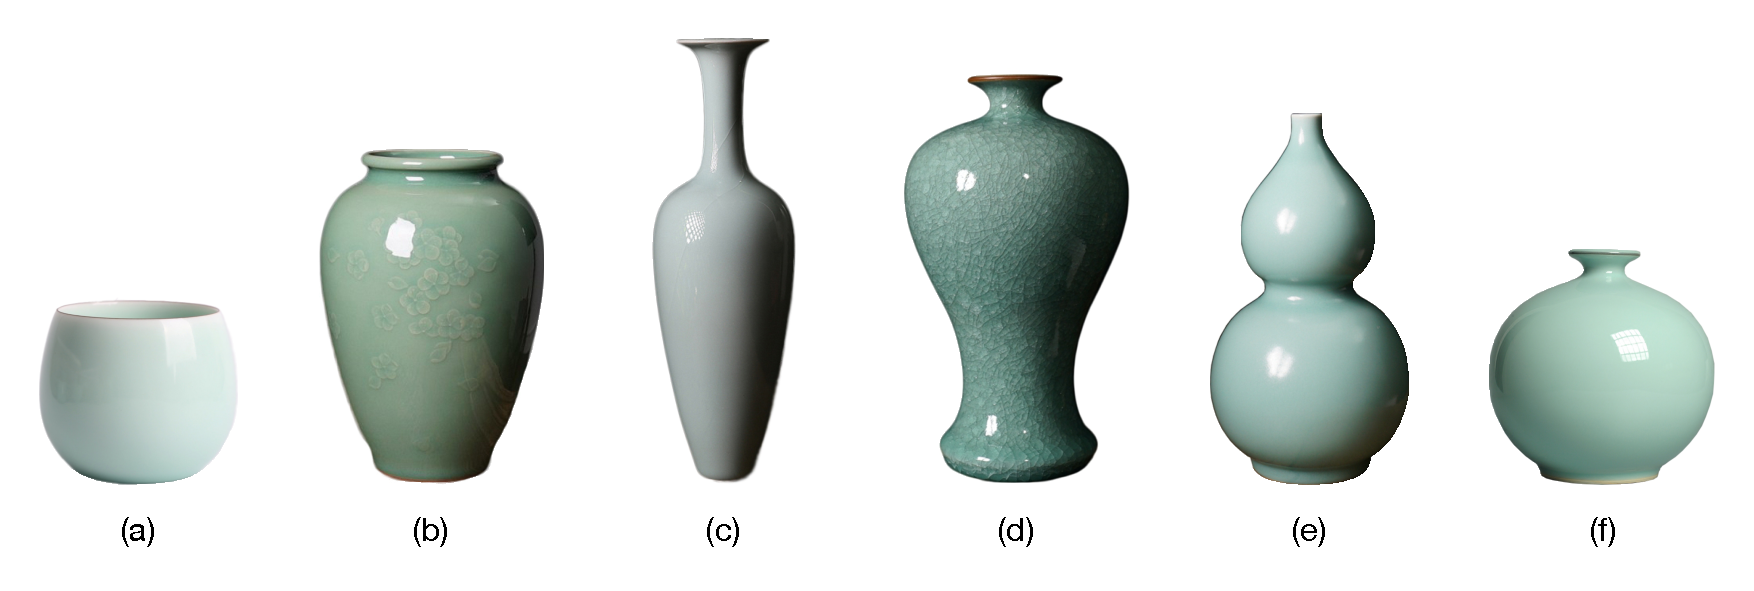
\includegraphics[width=\textwidth]{fig12}
\caption{The target shapes used in our user study, which have various heights and curvatures.}
\label{fig:target}
\end{figure*}

\paragraph{Practice} Each subject was given 15 minutes to get familiar with these systems (5 minutes for each). Subjects can ask questions whenever they need help.

\paragraph{Task 1} After the 15-minute practice of the three systems, each subject need to accomplish 3 tasks:

\textbf{T}\textsubscript{1}: Given a sequence of reference pot models as target shapes, the subjects were asked to create same pots from irregular generated meshes using RealPot. 

\textbf{T}\textsubscript{2}: Given reference pot models of the same order in \textbf{T}\textsubscript{1}, the subjects need to model these pots using Let's Create! Pottery on an iPad Pro.

\textbf{T}\textsubscript{3}: Given reference pot models of the same order in \textbf{T}\textsubscript{1} and \textbf{T}\textsubscript{2}, the subjects need to model these pots using Maya on a PC.

%[Task details]
When doing tasks \textbf{T}\textsubscript{1} to \textbf{T}\textsubscript{3}, a total of six target shapes were presented to subjects in a randomized sequence (Figure \ref{fig:pots}).
%%% TODO

%[NASA-TLX]
\paragraph{Questionnaire 1} After accomplishing each task, the subjects were asked to answer a questionnaire with six questions to measure the six dimensions of NASA-TLX, which includes physical demand, mental demand, temporal demand, effort, performance and frustration. 5 additional questions were asked after they finished all tasks.

%[Some explanations]
NASA-TLX has been chosen in our research because it is widely used in human factor studies which addressed questions about interface design and evaluation \cite{hart2006nasa}.
We selected NASA-TLX as a part of our questionnaire to assess user workload in the three systems.
Since the functionalities are different among the three systems, it is impossible and unfair to compare the interactions.
We intended to allow our subjects to experience those differences and similarities through these tasks and analyze which types of interactions and results were more attractive to them through our user study questions.

\paragraph{Task 2} After finishing tasks \textbf{T}\textsubscript{1} to \textbf{T}\textsubscript{3}, each subject need to accomplish 3 more tasks:

\textbf{T}\textsubscript{4}: Use RealPot to make a creative pottery model freely.

\textbf{T}\textsubscript{5}: Use Let's Create! Pottery to make a creative pottery model freely.

\textbf{T}\textsubscript{6}: Use Maya to make a creative pottery model freely.

\paragraph{Questionnaire 2} Each subject needs to answer the following questions after finishing tasks \textbf{T}\textsubscript{4} to \textbf{T}\textsubscript{6}:

\textbf{Q}\textsubscript{1}: Rank the three systems according to ease of learning from high to low.

\textbf{Q}\textsubscript{2}: Rank the three systems according to their supports for your imagination and creativity from high to low.

\textbf{Q}\textsubscript{3}: Rank the three systems according to your preference from high to low.


\subsubsection{Study Results}


%[basic introduction]
%Figure \ref{fig:boxplot} shows the boxplots of completion time and correlation coefficient for each target shape created in \textbf{T}\textsubscript{1}.
Figure \ref{fig:tlx} shows mean values of the six dimensions of NASA-TLX for \textbf{T}\textsubscript{1}, \textbf{T}\textsubscript{2} and \textbf{T}\textsubscript{3}.
Figure \ref{fig:ranking} shows the vote results of \textbf{Q}\textsubscript{1}, \textbf{Q}\textsubscript{2} and \textbf{Q}\textsubscript{3}, where we count a score of 3 for the system in the highest ranking and 1 for the system in the lowest ranking. 

%%%Fig%%% tlx
\begin{figure*}
	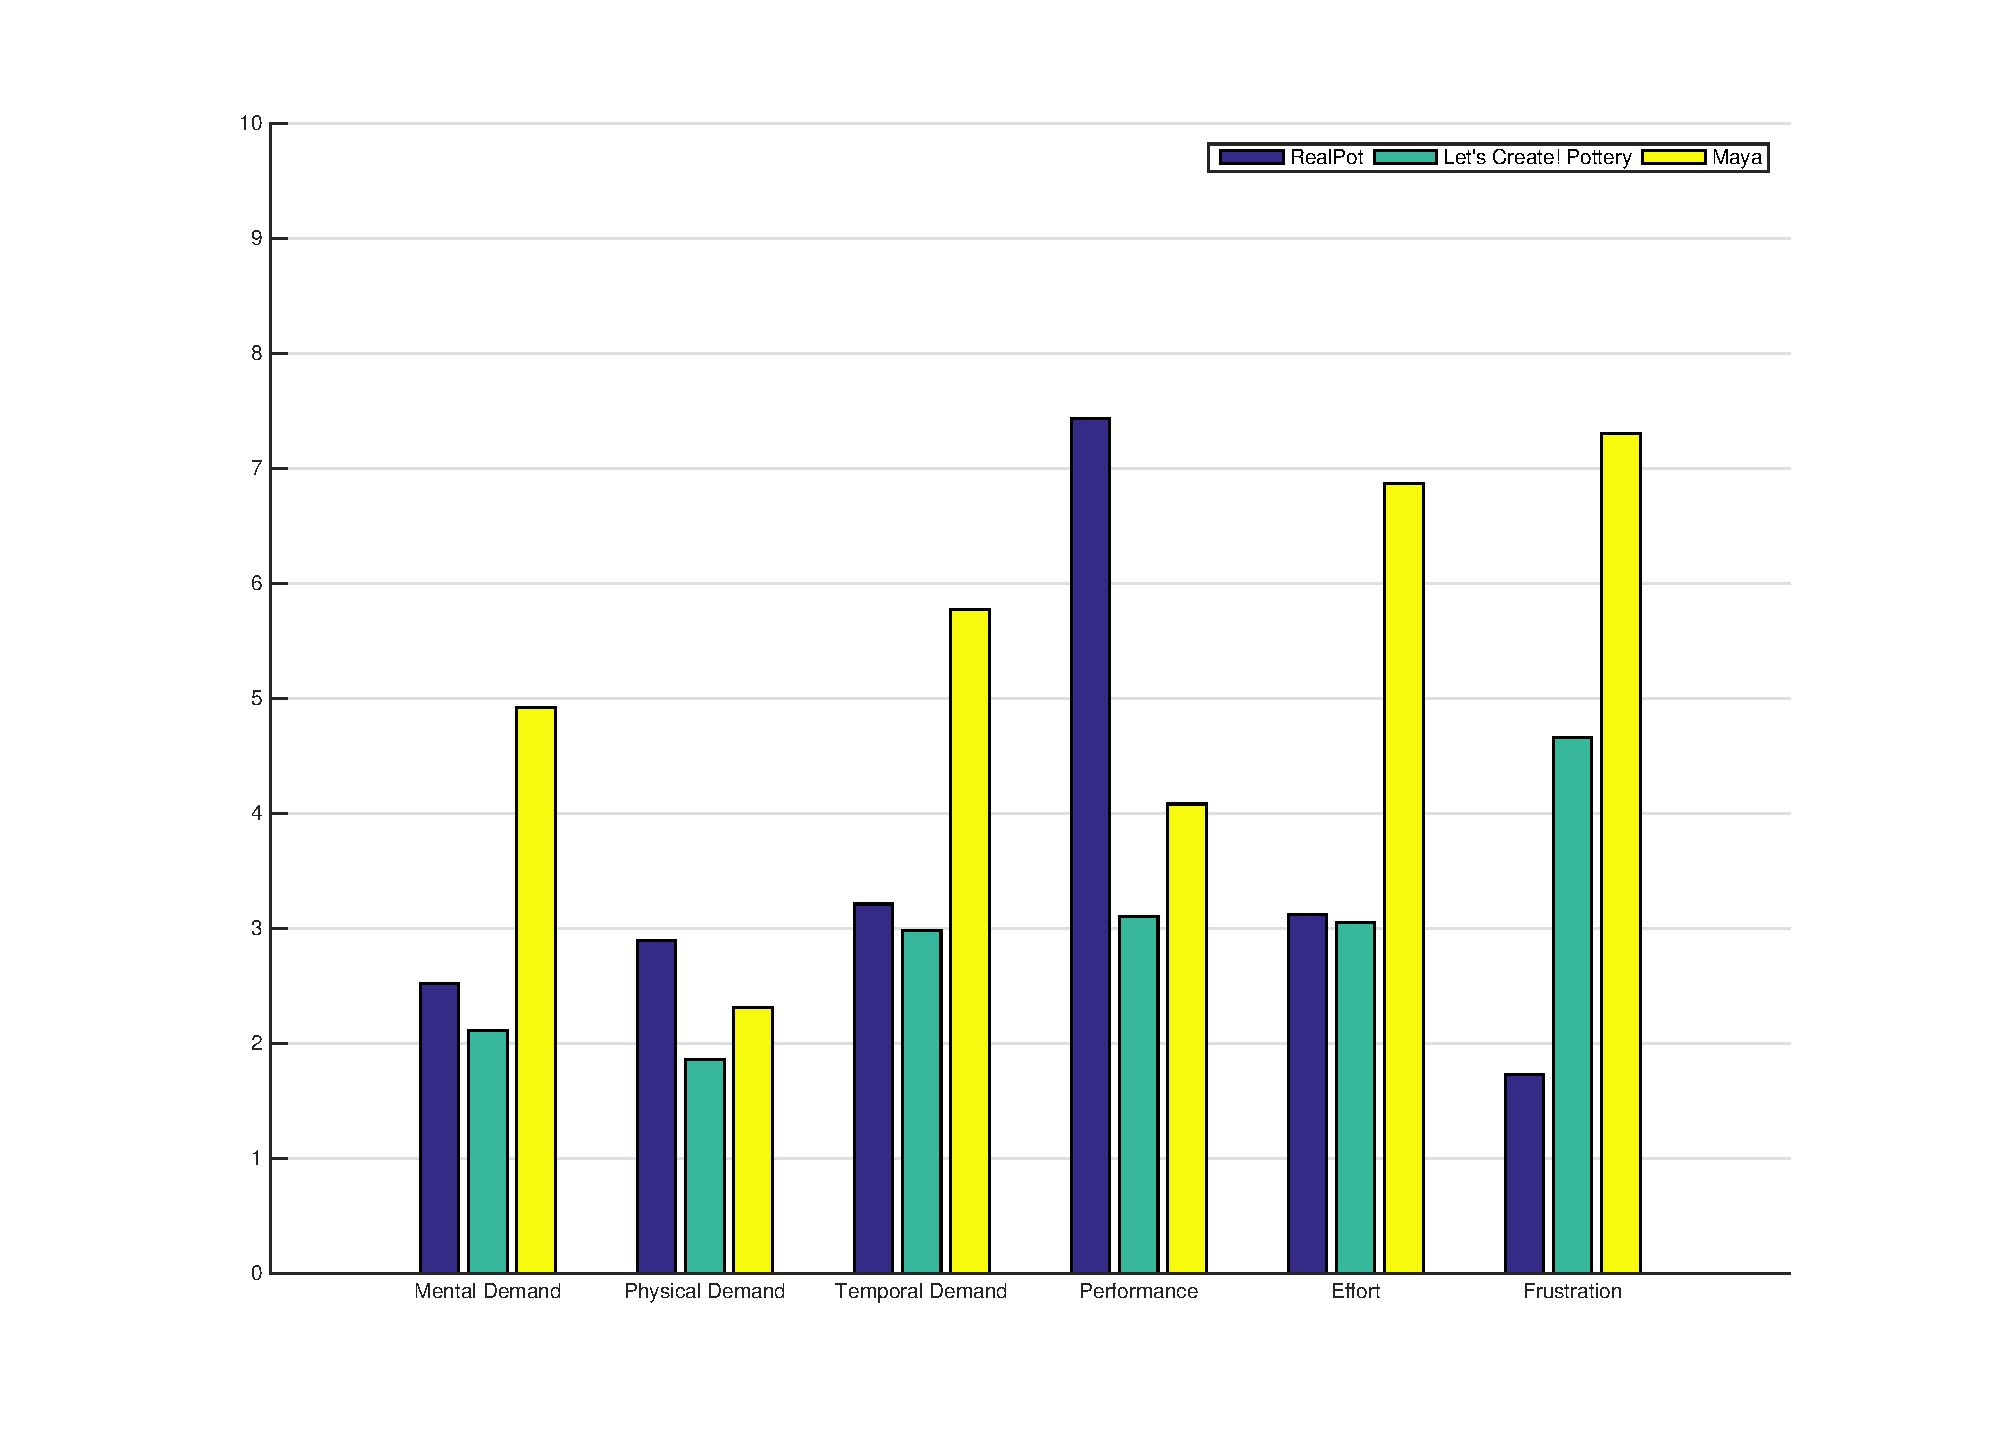
\includegraphics[width=\textwidth]{fig14.eps}
	\caption{Mean values of the six dimensions of NASA-TLX.}
	\label{fig:tlx}
\end{figure*}

%mental/physical/temporal
According to Figure \ref{fig:tlx}, we can get some findings. 
Firstly, the mental demand values of \textbf{T}\textsubscript{1} (M = 2.52) and \textbf{T}\textsubscript{2} (M = 2.11) were almost the same and much lower than the value of \textbf{T}\textsubscript{3} (M = 4.92). Similarly, the temporal demand value of \textbf{T}\textsubscript{3} (M = 5.77) was much higher than the values of \textbf{T}\textsubscript{1} (M = 3.21) and \textbf{T}\textsubscript{2} (M = 2.98). This indicated that RealPot and LCP were easier to use and less time-consuming than Maya. Unsurprisingly, the physical demand value of \textbf{T}\textsubscript{1} (M = 2.89) is slightly higher than \textbf{T}\textsubscript{2} (M = 1.86) and \textbf{T}\textsubscript{3} (M = 2.31), which means interactions based spatial movements are slightly more laborious than touchscreen and keyboard/mouse interactions.

%[Maya - hard]
Maya showed much higher values in effort (M = 6.87) and frustration (M = 7.30) and lower value in performance (M = 4.08) compared with RealPot and LCP.
Since most subjects in the user study have no 3D modeling software experience, the complex user interface in Maya makes it challenging for these novice users to memorize where to find the commands they need, rendering a high effort.
Although keyboard-mouse based interaction allows precise controls with low physical demand, many subjects struggled with selecting and manipulating vertices and faces accurately, which caused high user frustration. As a result, most subjects were not satisfied with their performances in \textbf{T}\textsubscript{3}.

%[LCP - limitation] [thickness smooth sharpness]
Surprisingly, we found that it was not as satisfied as we predicted for the subjects using LCP in \textbf{T}\textsubscript{2}, where the performance value (M = 3.10) is lower than we expected. This is due to the limitations in LCP: Although the interaction in LCP is easy to learn, some high curvature features (Figure \ref{fig:target}b, \ref{fig:target}d, \ref{fig:target}e and \ref{fig:target}f) cannot be reached due to LCP has a fixed deformation range. Moreover, subjects cannot modify the thickness of pots, which is another limitation of LCP. Thus, the frustration value (M = 4.66) are high during \textbf{T}\textsubscript{2}.

%%%Fig%%% ranking
\begin{figure*}
	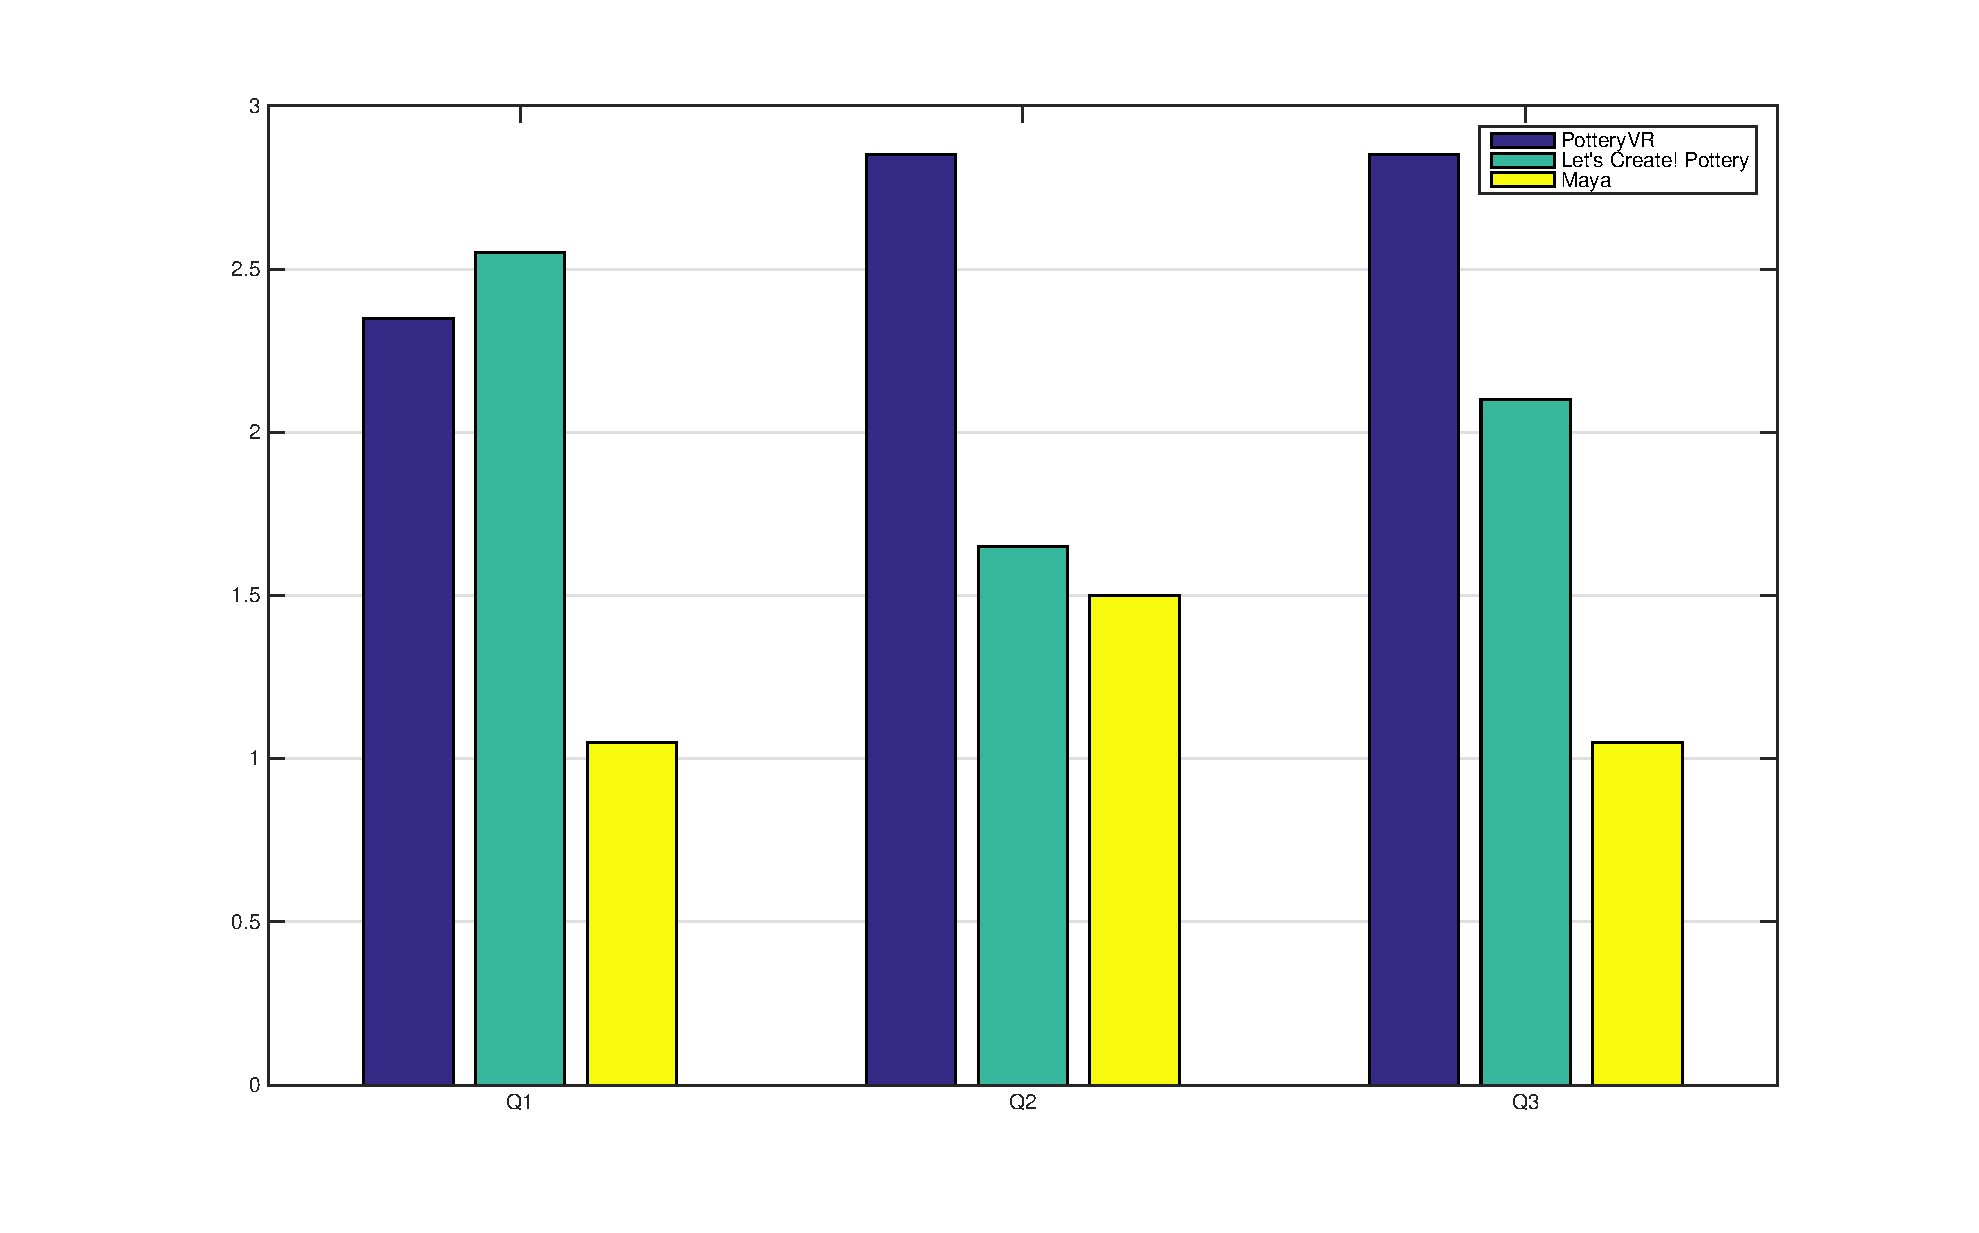
\includegraphics[width=0.75\textwidth]{fig15.eps}
	\caption{Mean ranking scores of Q1, Q2 and Q3.}
	\label{fig:ranking}
\end{figure*}

%[user preference][enjoyable and intuitive]
The voting results in Figure \ref{fig:ranking} demonstrated the ease of learning, the support of creativity and overall preference of the three systems.
%ease
Compared with the complex interfaces and the keyboard and mouse operations in Maya, RealPot and LCP provides simple interfaces and intuitive interactions, allowing users get familiar with the interaction with ease.
%creativity
In addition, most subjects considered RealPot stimulate their creativity and imagination the most. From their feedbacks, we found that spatial interactions in virtual reality context gave them a novel and realistic way to interact with virtual clay when using RealPot. Moreover, RealPot provides more powerful operations such as adjustable deformation range, thickness control and smoothing than LCP, allowing subjects creating characteristic shapes.

%overall-enjoyable, useful for training
In \textbf{Q}\textsubscript{3}, RealPot became the favorite virtual pottery system for the subjects. From user feedbacks, we found that RealPot provided the subjects with most enjoyable experience among the three systems, which also has a balance of having simple interfaces and useful functionalities. In addition, the natural bimanual interactions in RealPot are closely related to the operations in reality pottery, making it an ideal training simulation tool for pottery.




// The results show that ... FIG

// All participants commented that

// more comments from individuals

//FIG

\begin{figure*}
	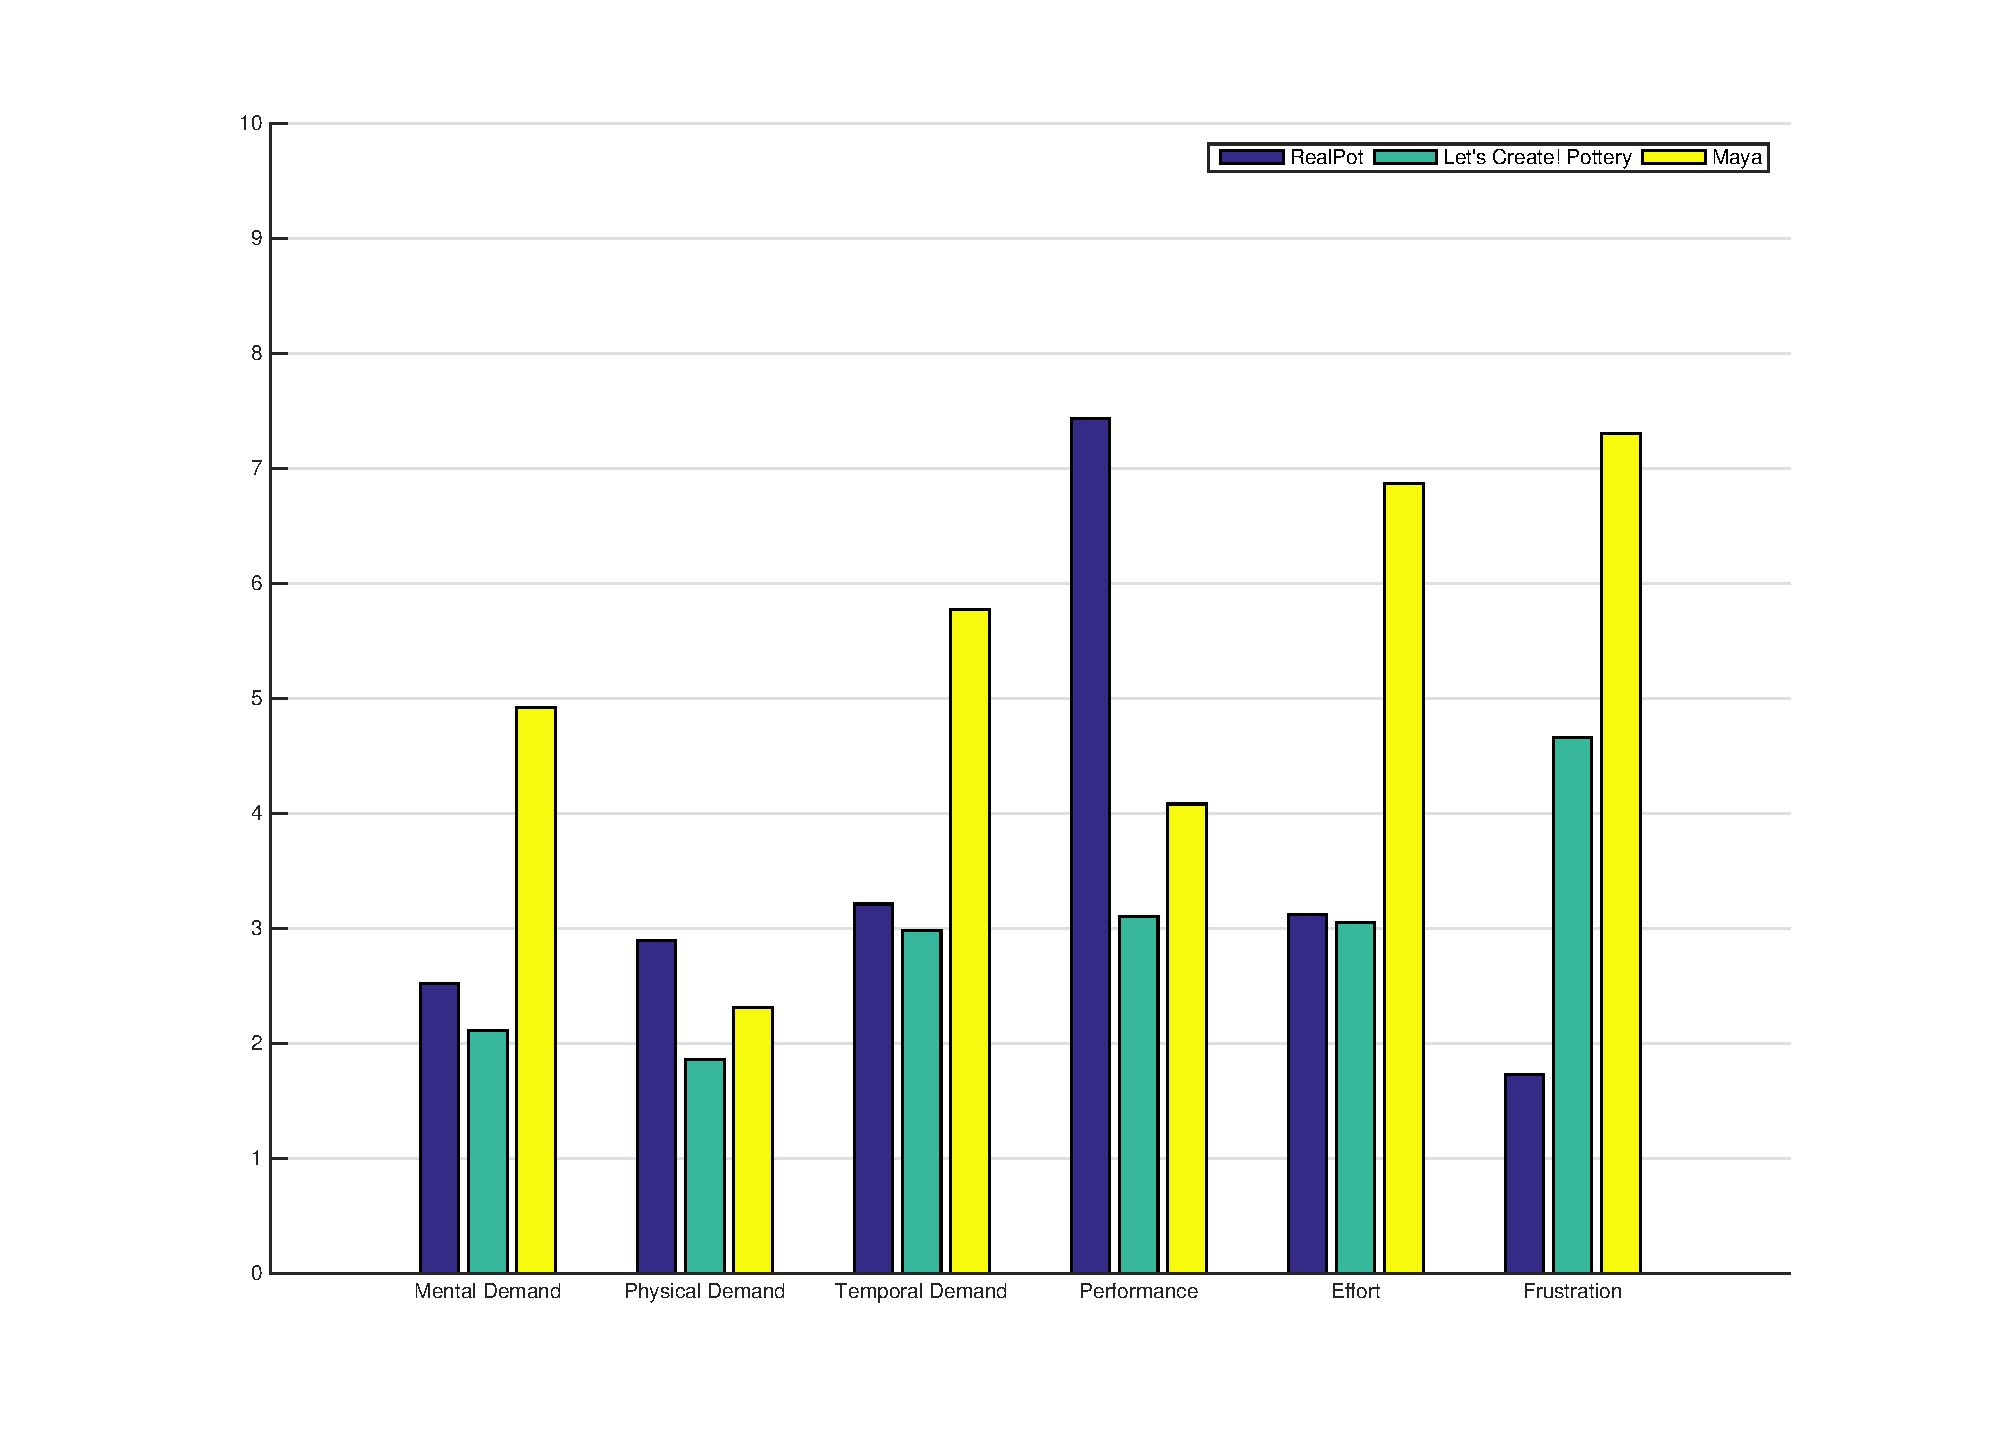
\includegraphics[width=\textwidth]{fig14.eps}
	\caption{user study 2 result here}
	\label{fig:u2r}
\end{figure*}


// From these results, the effectiveness of RealPot has been demostrated.



\subsection{User Study 2: vs other vp}
\label{sec:study2}

//In order to compare our system with prior CAD systems that can design virtual pottery on desktop and tablet platforms, we set up a comparative user study. We chose Autodesk Maya \cite{website:maya} as a representative of desktop modeling systems and Let's Create! Pottery (LCP) \cite{website:letspottery} as a representative of tablet pottery design systems.


\subsubsection{Evaluated Systems}

In user study 2, we investigated how our system compared with other virtual pottery systems.

// since these systems are hard to obtain, we use DigiClay as a representative bare-hand based pottery system.

// features in DigiClay

DigiClay is a virtual pottery system based on depth camera, with which the user can create pottery works using bare hands. //FIG

The interface 

The comparison is listed in the table.


\begin{figure*}
	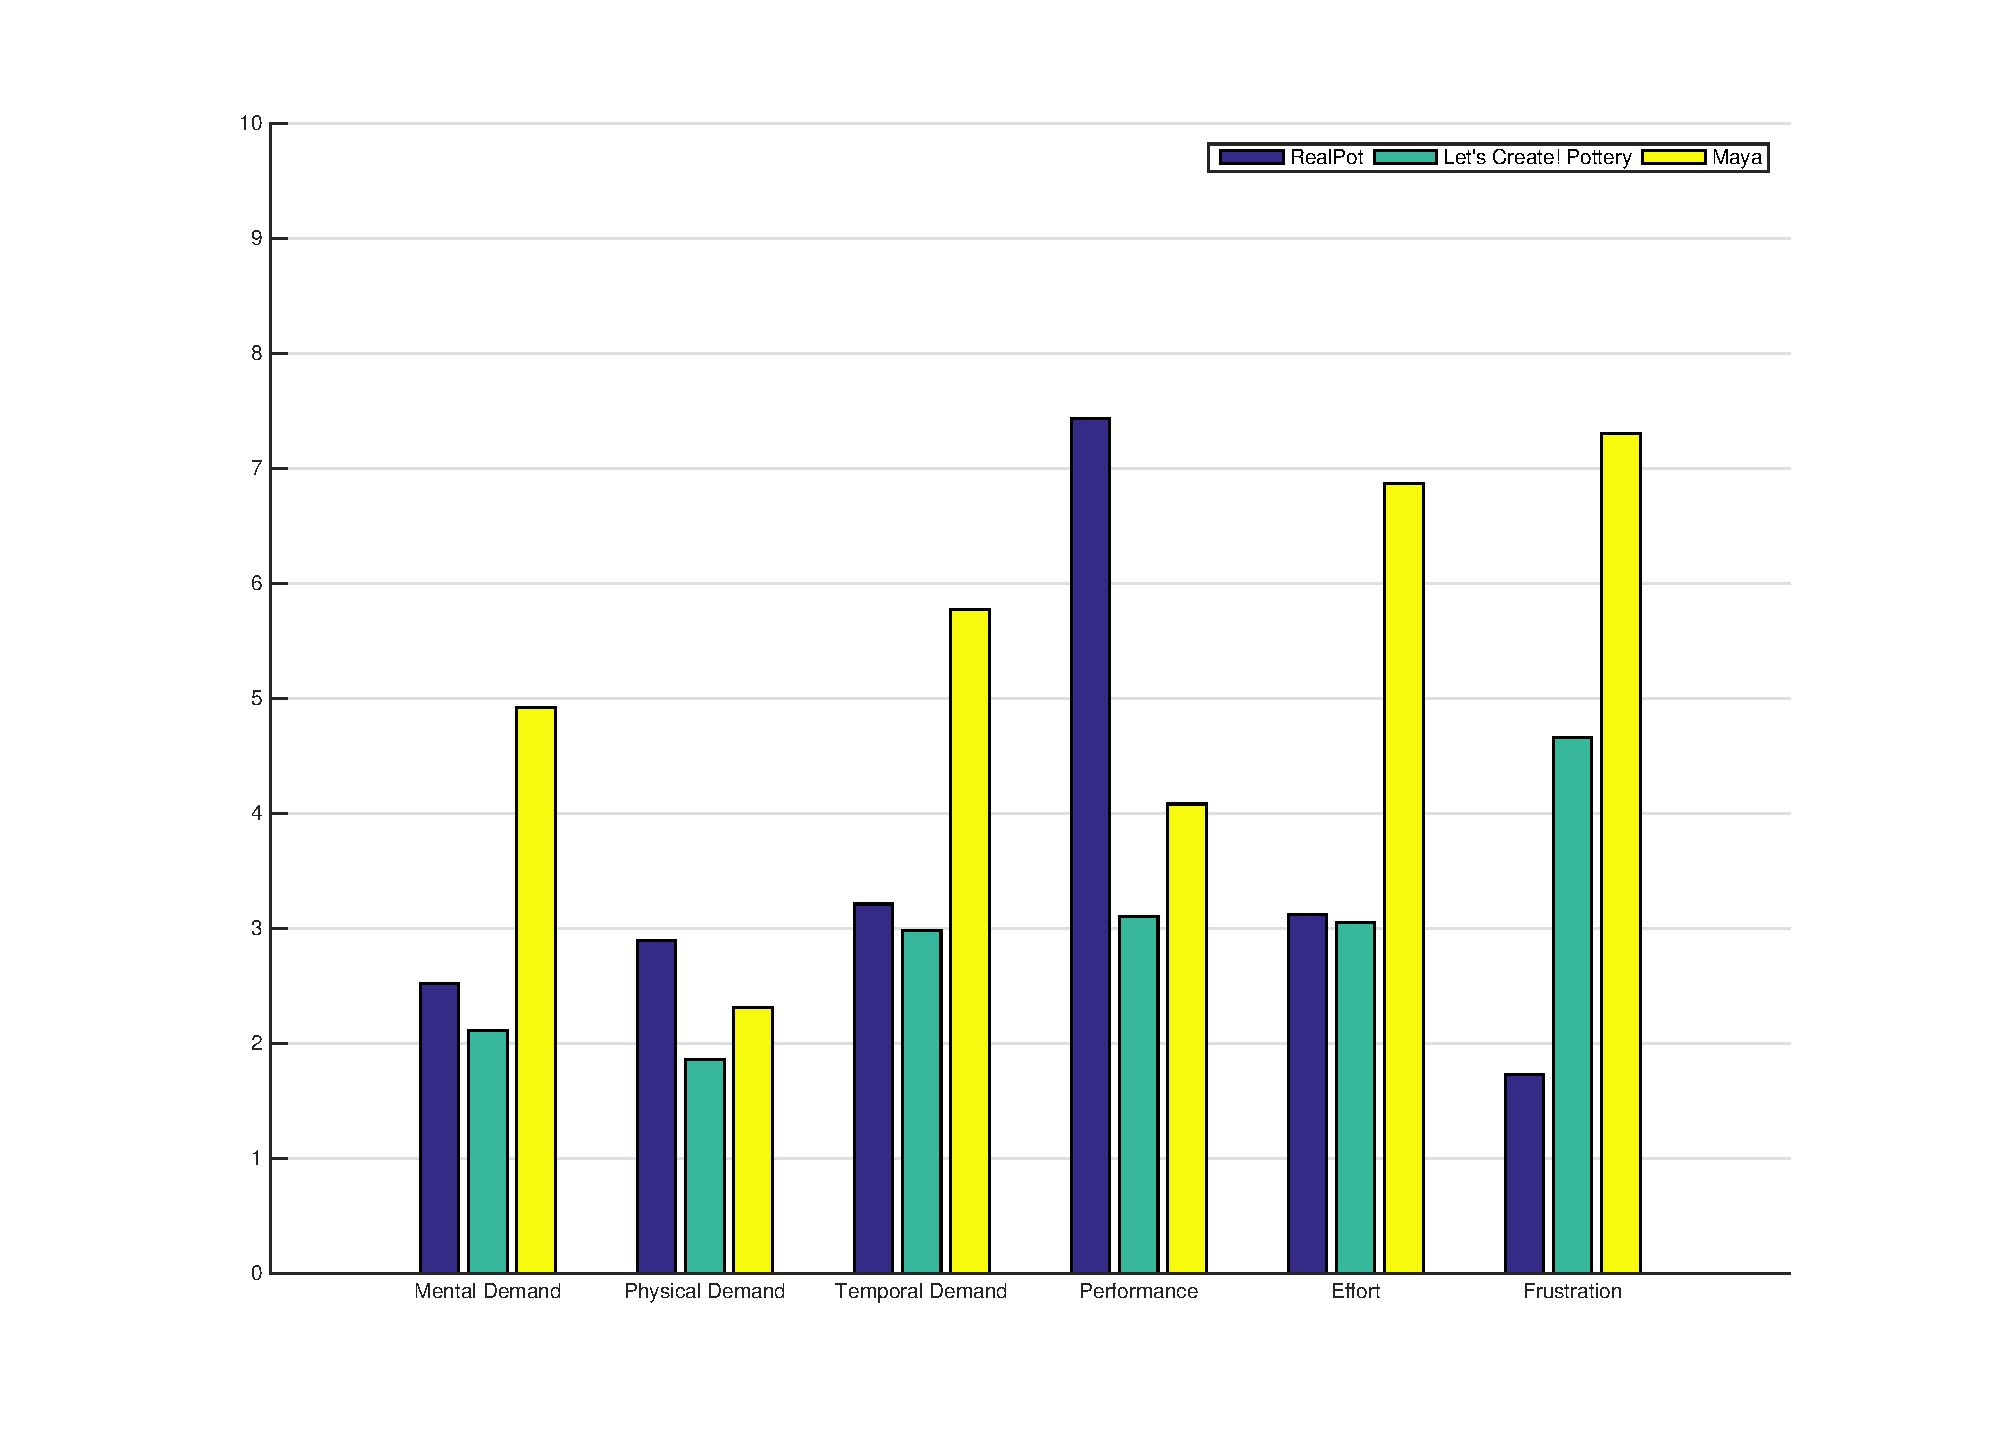
\includegraphics[width=\textwidth]{fig14.eps}
	\caption{DigiClay here}
	\label{fig:dc}
\end{figure*}

//TABLE

\begin{table}
% table caption is above the table
\caption{A comparison of two virtual pottery systems used in our user study.}
\label{tab:3}       % Give a unique label
% For LaTeX tables use
\begin{tabular}{llll}
\hline\noalign{\smallskip}
System & Input Device & Immersion & Haptic Feedback \\
\noalign{\smallskip}\hline\noalign{\smallskip}
RealPot & Hand-held Controllers & Yes & Yes \\
DigiClay & Depth Camera & No & No \\
\noalign{\smallskip}\hline
\end{tabular}
\end{table}


\subsubsection{Participants}

//participants

19 participants were participated in our user study, 10 males and 9 females, whose age ranged from 8 to 32 years. 8 of the subjects are familiar with VR systems (42.1\%); 2 of the subjects have experience with 3D modeling tools (10.5\%); 4 of the subjects have amateur pottery throwing experience in real life (21.1\%).


\subsubsection{Experimental Design and Procedure}

//tasks


Speed and accuracy are the most impoartant task performance metrics.

However, due to the implicit relationship between speed and accuracy, one can go faster but be less accurate, or can increase accuracy by decreasing speed.

it is impossible to do a task as quickly and precisely as possible.

// Accuracy first

//evaluation method (time, accuracy)



\subsubsection{Study Results}

For completion times, we performed a one-way ANOVA and the results showed different haptic models had a significant effect (F(1, 23) = 82.3503, p < 0.0001). 

For accuracy, we performed a one-way ANOVA and the results showed different haptic models had a significant effect (F(1, 23) = 82.3503, p < 0.0001). 

For subjective usability questionnaire, we performed a one-way ANOVA and the results showed different haptic models had a significant effect (F(1, 23) = 82.3503, p < 0.0001).


For completion times, we performed a one-way ANOVA and the results showed different haptic models had a significant effect (F(1, 23) = 82.3503, p < 0.0001). 

For accuracy, we performed a one-way ANOVA and the results showed different haptic models had a significant effect (F(1, 23) = 82.3503, p < 0.0001). 

For subjective usability questionnaire, we performed a one-way ANOVA and the results showed different haptic models had a significant effect (F(1, 23) = 82.3503, p < 0.0001).


\begin{table}
% table caption is above the table
\caption{User study 1 stats}
\label{tab:u1}       % Give a unique label
% For LaTeX tables use
\begin{tabular}{lllll}
\hline\noalign{\smallskip}
Axis Segments & Height Segments & Vertices & Triangles & Generation Time (ms)\\
\noalign{\smallskip}\hline\noalign{\smallskip}
60 & 100 & 12242 & 24120 & 21.48 \\
60 & 200 & 24242 & 48120 & 41.53 \\
\noalign{\smallskip}\hline
\end{tabular}
\end{table}


%[basic introduction]
%Figure \ref{fig:boxplot} shows the boxplots of completion time and correlation coefficient for each target shape created in \textbf{T}\textsubscript{1}.
Figure \ref{fig:tlx} shows mean values of the six dimensions of NASA-TLX for \textbf{T}\textsubscript{1}, \textbf{T}\textsubscript{2} and \textbf{T}\textsubscript{3}.

%%%Fig%%% tlx
\begin{figure*}
	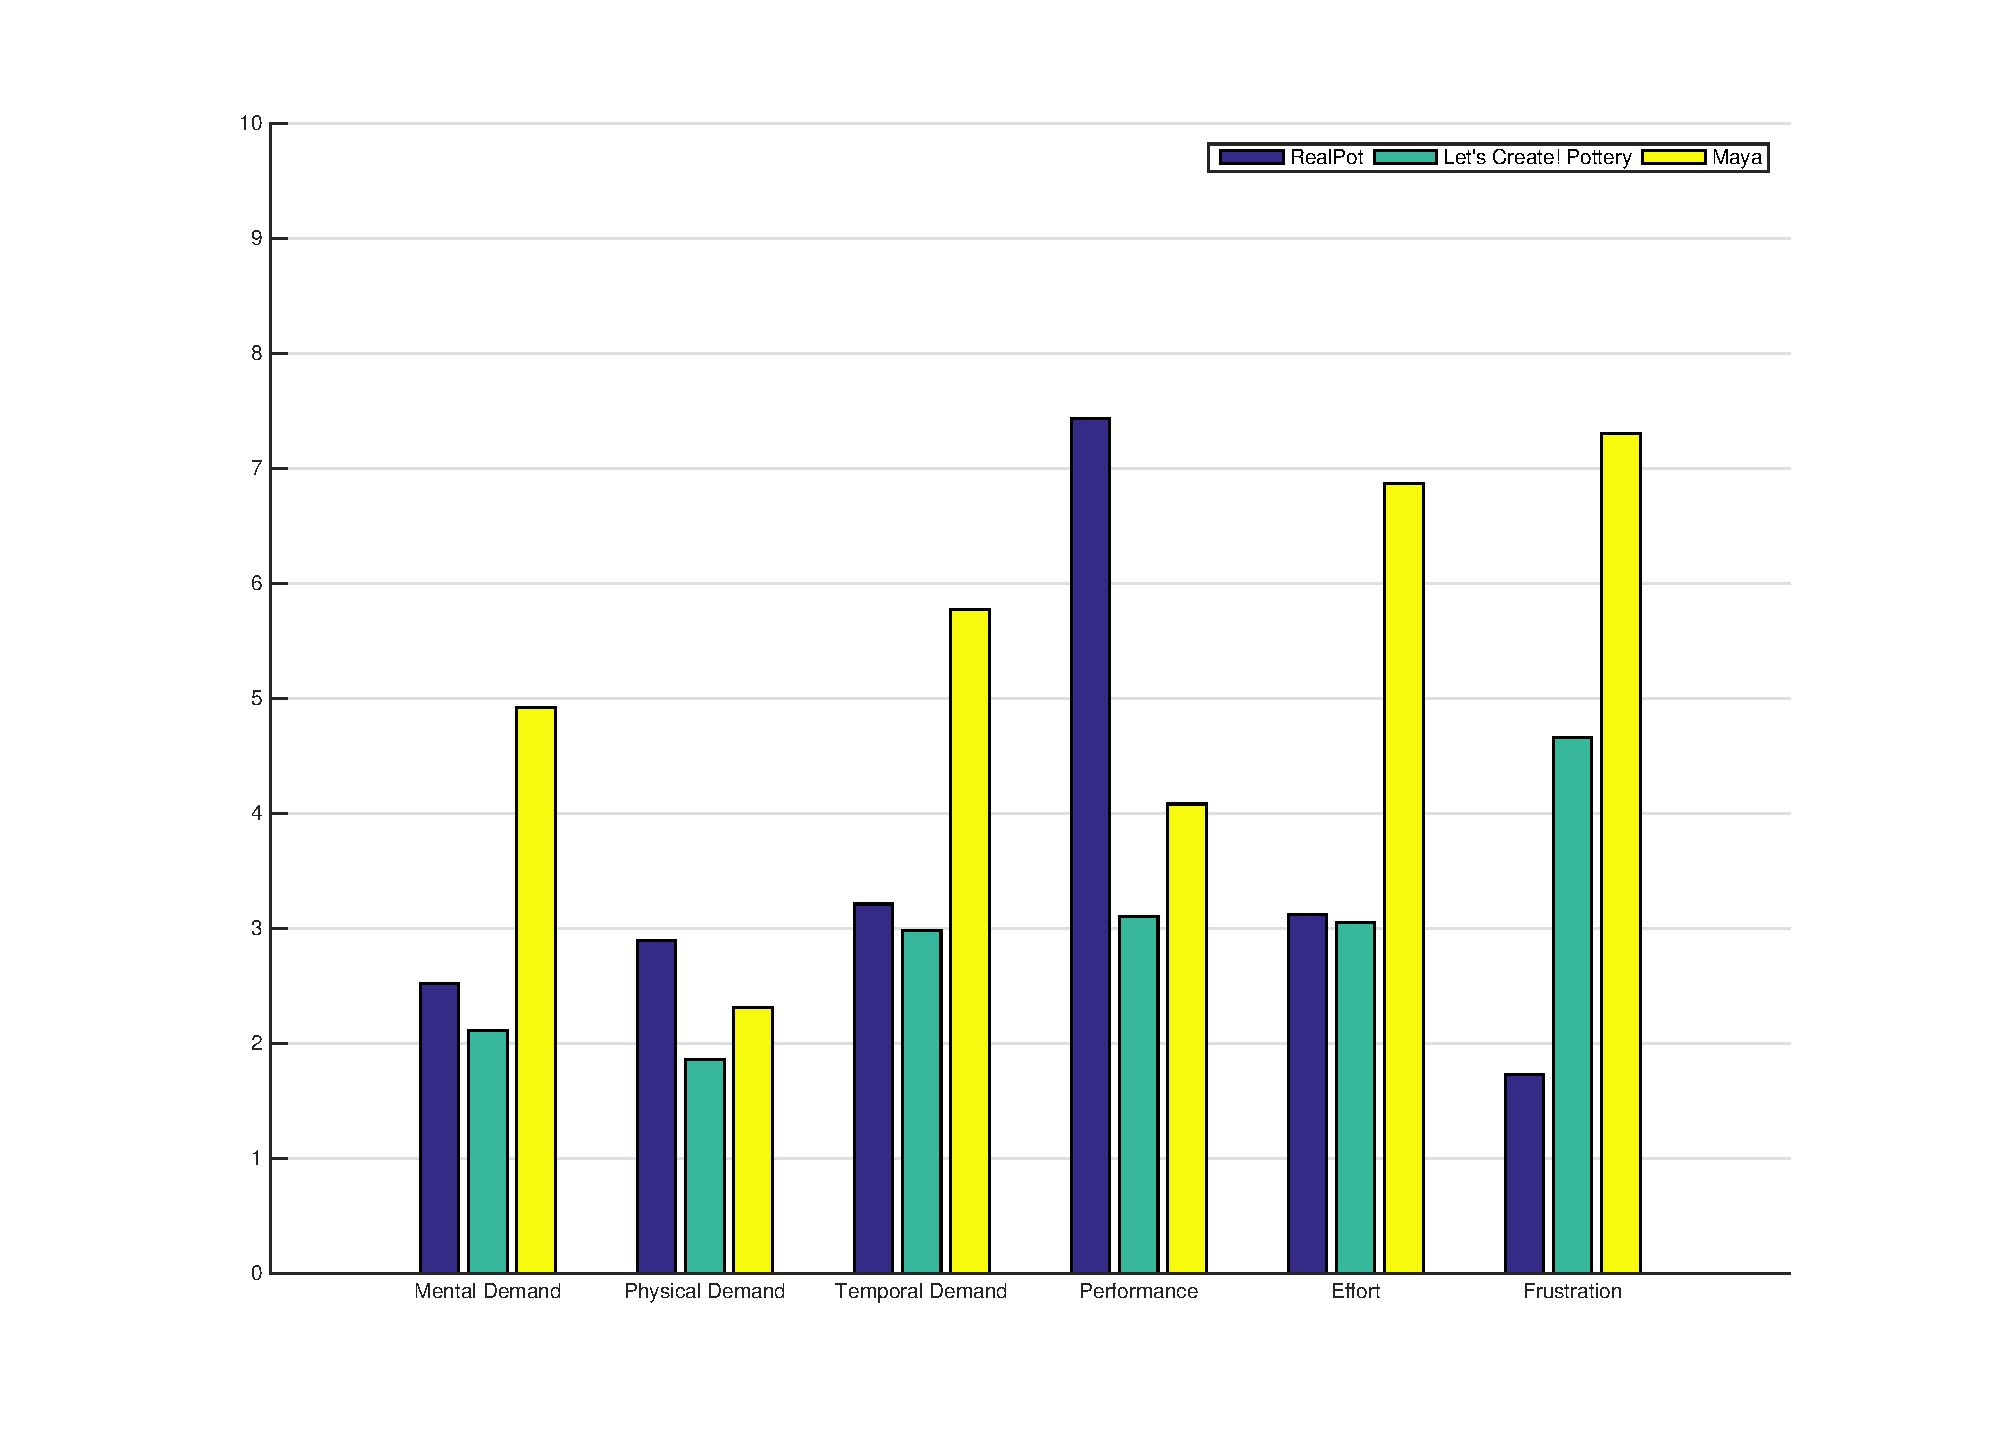
\includegraphics[width=\textwidth]{fig14.eps}
	\caption{Mean values of the six dimensions of NASA-TLX.}
	\label{fig:tlx}
\end{figure*}



